\documentclass[12pt]{beamer}
\newenvironment{ConCodigo}[1]
  {\begin{frame}[fragile,environment=ConCodigo]{#1}}
  {\end{frame}}
\graphicspath{{Imagenes/}{../Imagenes/}}
\usepackage[utf8]{inputenc}
\usepackage[spanish]{babel}
\usepackage{hyperref}
\usepackage{etex}
\reserveinserts{28}
\usepackage{amsmath}
\usepackage{amsthm}
\usepackage{mathtools}
\usepackage{multicol}
\usepackage{multirow}
\usepackage{tabulary}
%\usepackage{tabularx}
\usepackage{booktabs}
\usepackage{nccmath}
\usepackage{biblatex}
\usepackage{epstopdf}
\usepackage{graphicx}
\usepackage{siunitx}
\sisetup{scientific-notation=true}
%\usepackage{fontspec}
\usepackage{lmodern}
\usepackage{float}
\usepackage[format=hang, font=footnotesize, labelformat=parens]{caption}
\usepackage[autostyle,spanish=mexican]{csquotes}
\usepackage{standalone}
\usepackage{tikz}
\usepackage[siunitx]{circuitikz}
\usetikzlibrary{arrows,patterns,shapes}
\usetikzlibrary{decorations.markings}
\usetikzlibrary{arrows}
\usepackage{color}
%\usepackage{beton}
%\usepackage{euler}
%\usepackage[T1]{fontenc}
\usepackage[sfdefault]{roboto}  %% Option 'sfdefault' only if the base font of the document is to be sans serif
\usepackage[T1]{fontenc}
\renewcommand*\familydefault{\sfdefault}
\DeclareGraphicsExtensions{.pdf,.png,.jpg}
\usepackage{hyperref}
\renewcommand {\arraystretch}{1.5}
\newcommand{\python}{\texttt{python}}
\usefonttheme[onlymath]{serif}
\setbeamertemplate{navigation symbols}{}
\usetikzlibrary{patterns}
\usetikzlibrary{decorations.markings}
\tikzstyle{every picture}+=[remember picture,baseline]
%\tikzstyle{every node}+=[inner sep=0pt,anchor=base,
%minimum width=2.2cm,align=center,text depth=.15ex,outer sep=1.5pt]
%\tikzstyle{every path}+=[thick, rounded corners]
\setbeamertemplate{caption}[numbered]
\newcommand{\ptm}{\fontfamily{ptm}\selectfont}
%Se usa la plantilla Warsaw modificada con spruce
\mode<presentation>
{
  \usetheme{Warsaw}
  \setbeamertemplate{headline}{}
  \useoutertheme{default}
  \usecolortheme{beaver}
  \setbeamercovered{invisible}
}
\AtBeginSection[]
{
\begin{frame}<beamer>{Contenido}
\normalfont\mdseries
\tableofcontents[currentsection]
\end{frame}
}

\usepackage{listings}
\lstset{ %
language=Python,                % choose the language of the code
basicstyle=\small,       % the size of the fonts that are used for the code
numbers=left,                   % where to put the line-numbers
numberstyle=\small,      % the size of the fonts that are used for the line-numbers
stepnumber=1,                   % the step between two line-numbers. If it is 1 each line will be numbered
numbersep=5pt,                  % how far the line-numbers are from the code
backgroundcolor=\color{white},  % choose the background color. You must add \usepackage{color}
showspaces=false,               % show spaces adding particular underscores
showstringspaces=false,         % underline spaces within strings
showtabs=false,                 % show tabs within strings adding particular underscores
frame=single,   		% adds a frame around the code
tabsize=2,  		% sets default tabsize to 2 spaces
captionpos=b,   		% sets the caption-position to bottom
breaklines=true,    	% sets automatic line breaking
breakatwhitespace=false,    % sets if automatic breaks should only happen at whitespace
escapeinside={\%},          % if you want to add a comment within your code
stringstyle =\color{magenta},
keywordstyle = \color{blue},
commentstyle = \color{green},
identifierstyle = \color{red}
}
%\usepackage{siunitx}
%\usepackage[american,cuteinductors,smartlabels]{circuitikz}
%\usetikzlibrary{calc}
\title{Ecuaciones diferenciales ordinarias 3}
\subtitle{Curso de Física Computacional}
\author{M. en C. Gustavo Contreras Mayén}
\begin{document}
\maketitle
\fontsize{14}{14}\selectfont
\spanishdecimal{.}
\begin{frame}{Contenido}
\tableofcontents[pausesections]
\end{frame}
\section{Ejercicios avanzados.}
\begin{frame}
\frametitle{Ejecicio}
La corriente eléctrica de un circuito $RLC$ en serie, satisface la ecuación\\
\begin{equation} \label{eq:ecuacion1}
	L \frac{di}{dt}+ Ri+ \frac{1}{C} \int_{0}^{t} i(t') dt' +\frac{1}{C}q(0)= E(t), \hspace{0.75cm} t>0 
\end{equation}
cuando el circuito se cierra en el instante $t=0$, se tiene que $i=i(t)$ es la corriente, $R$ es la resistencia, $L,C,E$ vienen dadas por: $L=200H$, $C=0.001F$, $E(t)=1V$ para $t>0$.
\end{frame}
\begin{frame}
\begin{center}
\begin{circuitikz}
\draw
    (0,0)
        to[sV, l=$V_{s}$] ++(0,3)
        to[short] ++(1,0)
        to[cspst, o-o] ++(1,0)
        to[short] ++(1,0)
        to[L, l=$L$] ++(1,0)
        to[short] ++(1,0)
        to[short] ++(0,-1)
        to[C, l=$C$] ++(0,-1)
        to[short] ++(0,-1)
        to[short] ++(-1,0)
        to[R, l=$R$] ++(-1,0) --(0,0);
\end{circuitikz}
\end{center}
Las condiciones iniciales son $q(0)=0$ (carga inicial del condensador), $i(0)=0$. 
\end{frame}
\begin{frame}
Calcular la corriente para $0 \leq t \leq 5$ segundos y el factor de amortiguamiento y la frecuencia de oscilación del circuito $RLC$ para los siguientes valores de R:\\
\begin{enumerate}
	\item $R = 0 \hspace{0.1cm} \Omega$
	\item $R = 50 \hspace{0.1cm} \Omega$
	\item $R = 100 \hspace{0.1cm} \Omega$
	\item $R = 300 \hspace{0.1cm} \Omega$
\end{enumerate}
\end{frame}
\begin{frame}
Si definimos
\begin{equation}\label{eq:ecuacion2}
	q(t) = \int_{0}^{t'} i(t') dt'
\end{equation}
derivando la expresión anterior
\begin{equation}\label{eq:ecuacion3}
	\dfrac{d}{dt}q(t) = i(t), \hspace{1.5cm} q(0)=0
\end{equation}
Sustituimos en la ecuació inicial, para re-escribir
\fontsize{12}{12}\selectfont
\begin{equation}\label{eq:ecuacion4}
	\dfrac{d}{dt}i(t) = -\dfrac{R}{L}i(t) - \dfrac{1}{LC} q(t) + \dfrac{1}{LC}q(0) + \dfrac{E(t)}{L}, i(0)=0 
\end{equation}
La ecuación (\ref{eq:ecuacion1}) se transformó en un sistema de dos EDO de primer orden: las ecuaciones (\ref{eq:ecuacion3}) y (\ref{eq:ecuacion4}).
\end{frame}
\begin{frame}
\frametitle{Solución gráfica con $R=0 \Omega$}
\begin{figure}
	\centering
	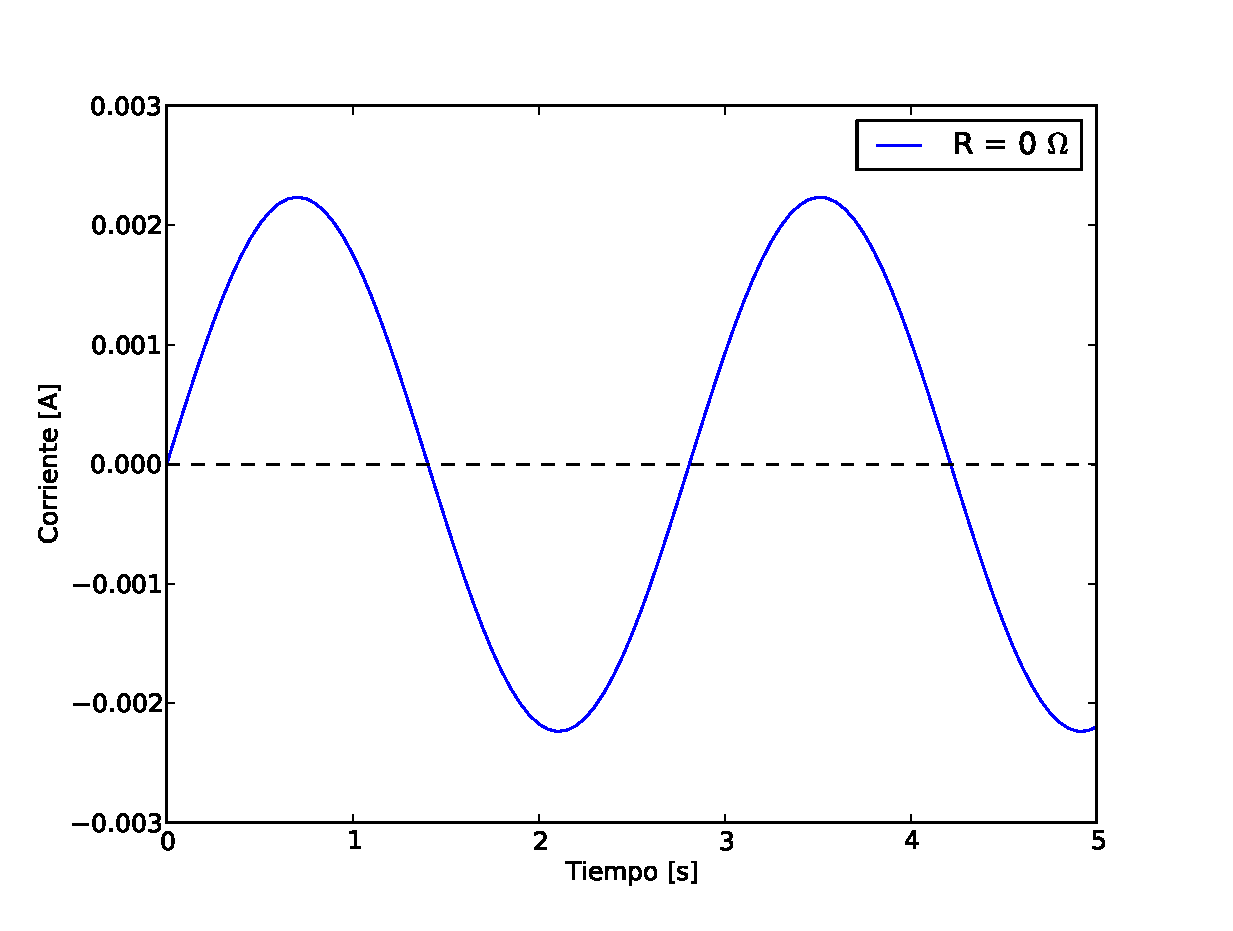
\includegraphics[scale=0.5]{SistemaElecRK4_01.eps} 
\end{figure}
\end{frame}
\begin{frame}
\frametitle{Solución gráfica con $R=50 \Omega$}
\begin{figure}
	\centering
	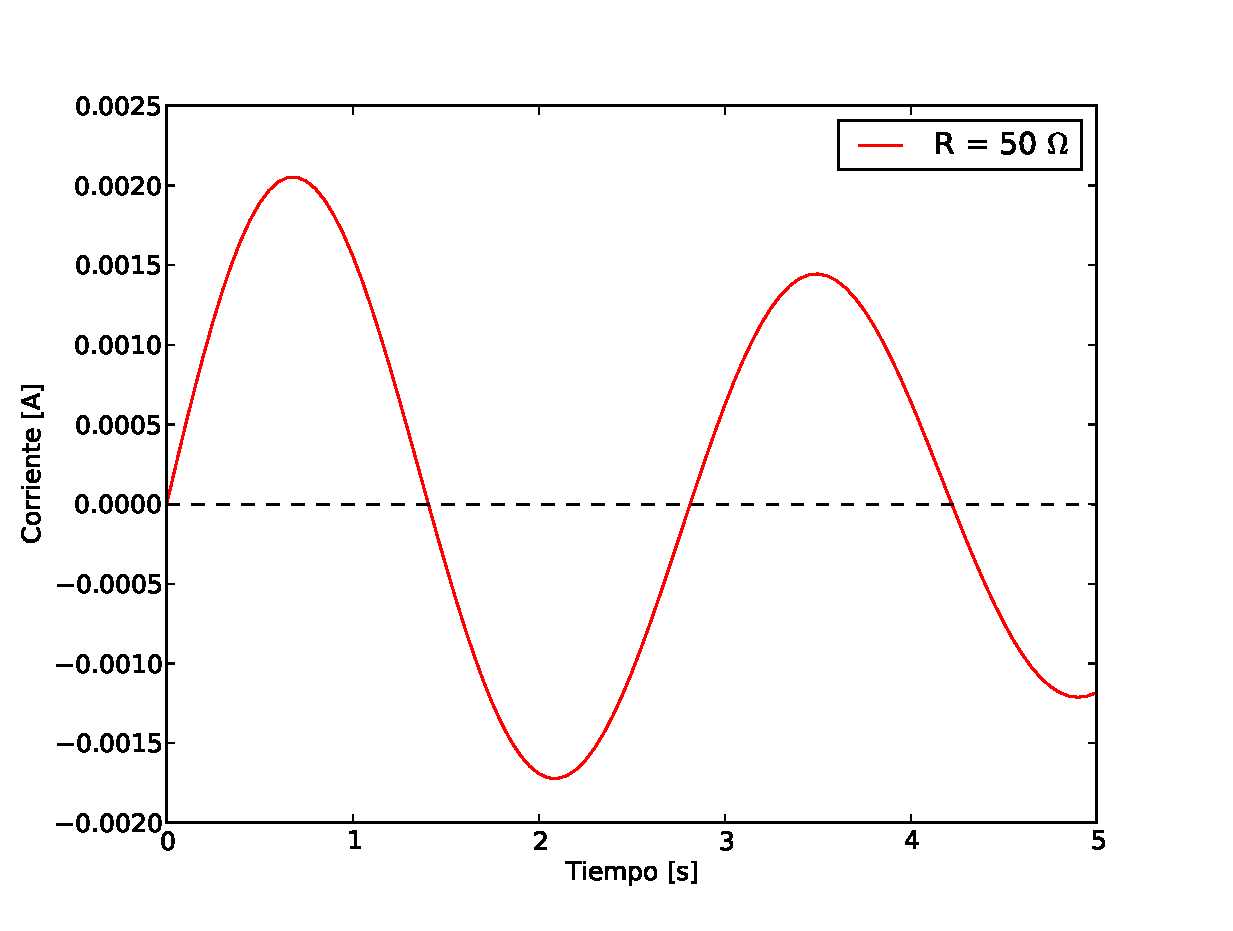
\includegraphics[scale=0.5]{SistemaElecRK4_02.eps} 
\end{figure}
\end{frame}
\begin{frame}
\frametitle{Solución gráfica con $R=100 \Omega$}
\begin{figure}
	\centering
	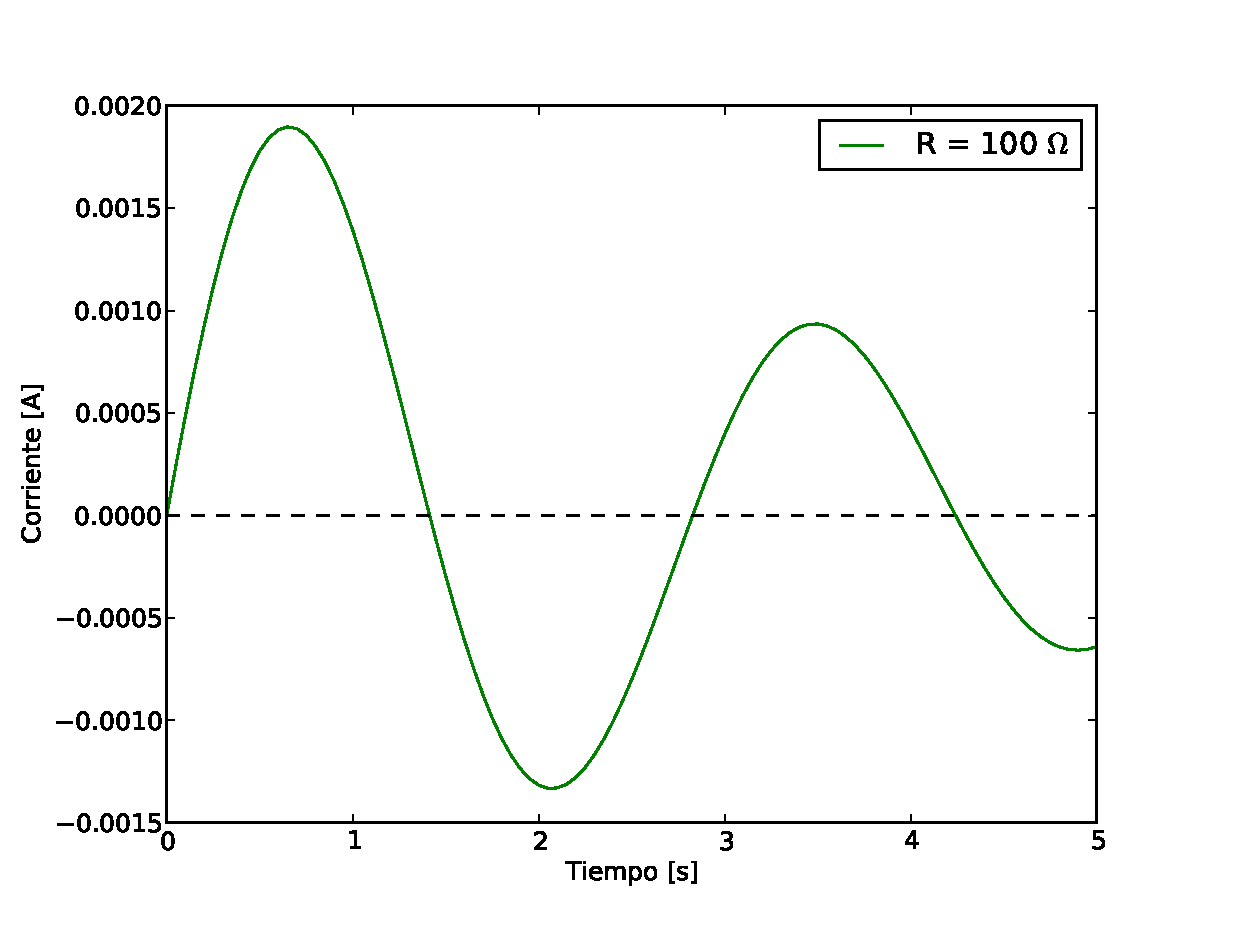
\includegraphics[scale=0.5]{SistemaElecRK4_03.eps} 
\end{figure}
\end{frame}
\begin{frame}
\frametitle{Solución gráfica con $R=300 \Omega$}
\begin{figure}
	\centering
	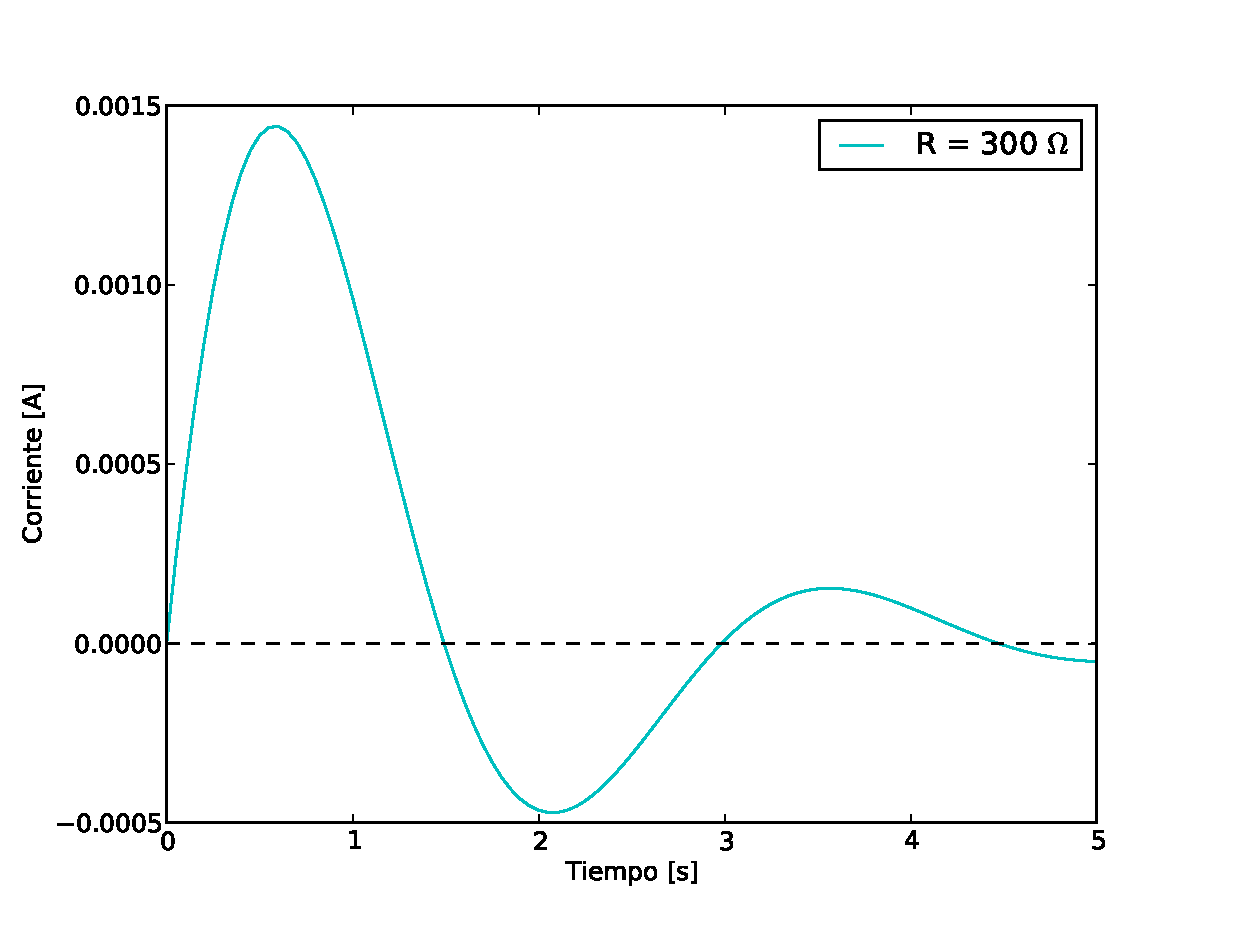
\includegraphics[scale=0.5]{SistemaElecRK4_04.eps} 
\end{figure}
\end{frame}
\begin{frame}
\frametitle{Solución gráfica con valores de $R$ superpuestos}
\begin{figure}
	\centering
	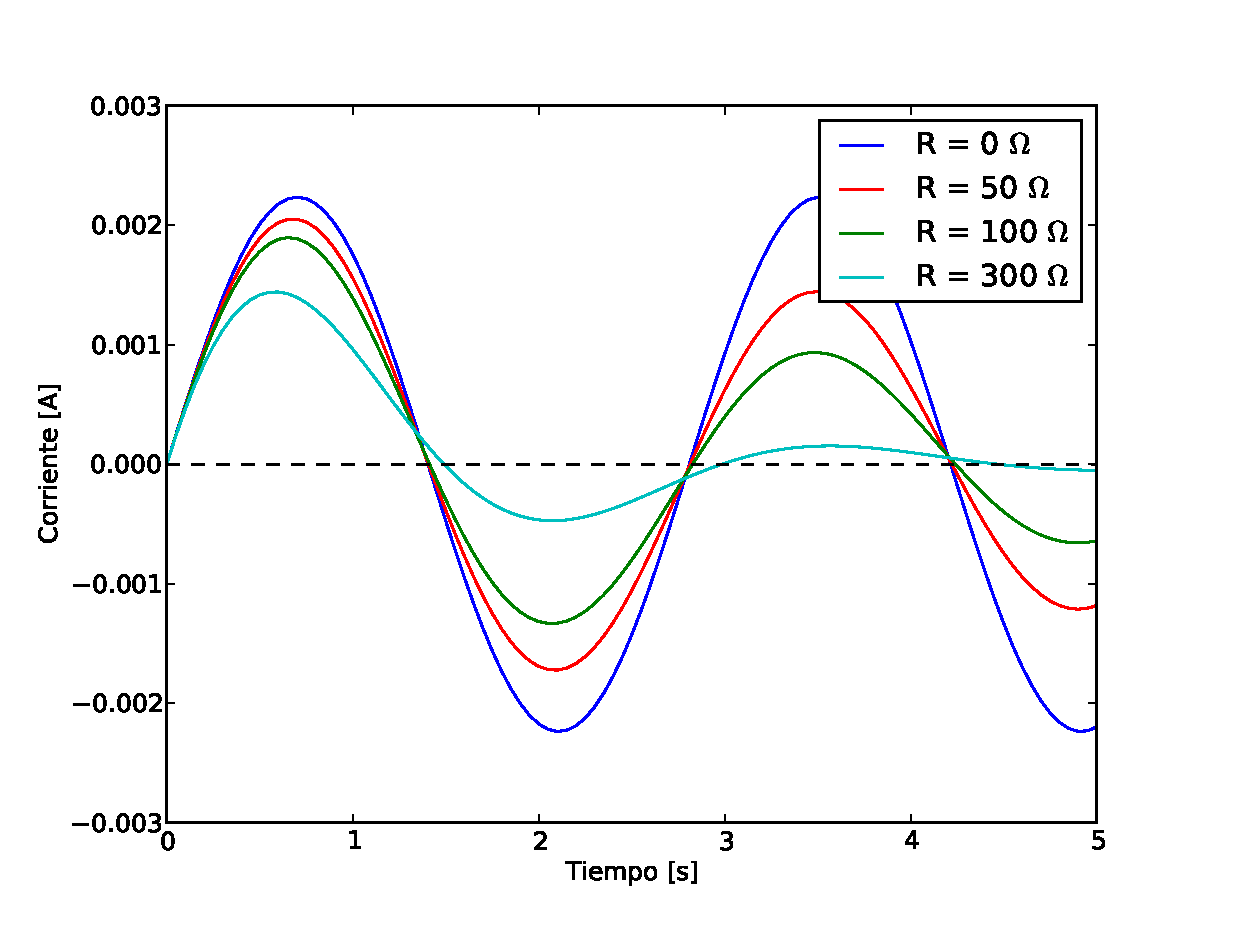
\includegraphics[scale=0.5]{SistemaElecRK4_05.eps} 
\end{figure}
\end{frame}
\begin{frame}[fragile]
\frametitle{Ejercicio 2}
En la figura se muestra un sistema de tres masas. Los desplazamientos de estas tres masas satisfacen las ecuaciones dadas por:
\fontsize{12}{12}\selectfont
\begin{eqnarray*} 
	M_{1} y''_{1} + B_{1} y'_{1} + K_{1} y_{1} - B_{1} y'_{2} - K_{2}y_{2} & = & F_{1}(t) \\
	-B_{1} y'_{1} - K_{1} y_{1} + M_{2} y''_{2} + B_{1} y'_{2} + (K_{1} + K_{2}) y_{2} - K_{2} y_{3} & = & 0 \\
	-K_{2} y_{2} + M_{3} y''_{3} + B_{2} y'_{3} + (K_{2} + K_{3}) y_{3} & = & F_{3}(t) 
\end{eqnarray*}
\begin{tikzpicture}[scale=0.6, font=\small]
	\tikzstyle{spring}=[thick,decorate,decoration={zigzag,pre length=0.1cm,post
  length=0.1cm,segment length=6}]
	\draw [->,thick] (-1,1.6) -- node [above, midway] {$F_{1}$}(0,1.6);
	\draw (0,-0.4) -- (0,0);
	\draw (-0.5,-0.1) -- (-0.5,-0.4);
	\draw [->](-0.5,-0.25) -- node [midway, below] {$y_{1}$}(0,-0.25);
	\draw (0,0) rectangle node {$M_{1}$}(2,2);
	\draw[spring] (2,1.7) -- node [above] {$k_{1}$} (4,1.7);
	\draw (2,0.5) -- (2.6,0.5);
	\draw (2.6,0.1) -- (2.6,0.9);
	\draw (2.6,0.1) -- (3,0.1);
	\draw (2.8,-0.3) node {$B_{1}$};
	\draw (2.6,0.9) -- (3.0,0.9);
	\draw (2.8,0.3) -- (2.8,0.7);
	\draw (2.8,0.5) -- (4,0.5);
	\draw (4,-0.4) -- (4,0);
	\draw (3.5,-0.1) -- (3.5,-0.4);
	\draw [->](3.5,-0.25) -- node [midway, below] {$y_{2}$}(4,-0.25);
	\draw (4,0) rectangle node {$M_{2}$}(6,2);
	\draw [spring] (6,1) -- node [below] {$k_{2}$} (8,1);
	\draw [->,thick] (7,1.6) -- node [above, midway] {$F_{3}$}(8,1.6);
	\draw (8,-0.4) -- (8,0);
	\draw (7.5,-0.1) -- (7.5,-0.4);
	\draw [->](7.5,-0.25) -- node [midway, below] {$y_{3}$}(8,-0.25);
	\draw (8,0) rectangle node {$M_{3}$} (10,2);
	\draw[spring] (10,1.7) -- node [above] {$k_{3}$} (12,1.7);
	\draw (10,0.5) -- (10.6,0.5);
	\draw (10.6,0.1) -- (10.6,0.9);
	\draw (10.6,0.1) -- (11,0.1);
	\draw (10.8,-0.3) node {$B_{2}$};
	\draw (10.6,0.9) -- (11.0,0.9);
	\draw (10.8,0.3) -- (10.8,0.7);
	\draw (10.8,0.5) -- (12,0.5);
	\draw [pattern=north east lines] (12,-0.5) rectangle (14,3);
\end{tikzpicture}
\end{frame}
\begin{frame}
Las constantes y condiciones iniciales son
\fontsize{12}{12}\selectfont
\begin{tabbing}
$K_{1} = K_{2} = K_{3} = 1$ \hspace{1.2cm} \= (constantes de los resortes, kgm/$s^{2}$) \\
$M_{1} = M_{2} = M_{3} = 1$ \> (masa, kg) \\
$F_{1}(t) = 1, F_{3}(t) = 0$ \> (fuerza, N) \\
$B_{1} = B_{2} =0.1$ \> (coeficientes de amortiguamiento, kg/s) \\
\\
$y_{1}(0) = y'_{1}(0) = y_{2}(0) = y'_{2}(0) = y_{3}(0) = y'_{3}(0) = 0$ \\
\> (condiciones iniciales)
\end{tabbing}
Resuelve y grafica las ecuaciones anteriores mediante RK4, para $0 \leq t \leq 30$ segundos y $h=0.1$ \\
\end{frame}
\begin{frame}
Hint: Definiendo
\[ y_{4} = y'_{1}, \hspace{1cm} y_{5} = y'_{2}, \hspace{1cm} y_{6} = y'_{3} \]
La ecuación inicial se escribe como un conjunto de seis EDO de primer orden, de la siguiente manera:
\begin{eqnarray*}
y'_{1} & = & y_{4} \\
y'_{2} & = & y_{5} \\
y'_{3} & = & y_{6} \\
y'_{4} & = & \left[ -B_{1} y_{4} - K_{1} y_{1} + B_{1} y_{5} + K_{2} y_{2} + F_{1} \right] / M_{1} \\
y'_{5} & = & \left[ B_{1} y_{4} + K_{1} y_{1} - B_{1} y_{5} - \left( K_{1} + K_{2} \right) y_{2} + K_{2} y_{3} \right] / M_{2}\\
y'_{6} & = & \left[ K_{2} y_{2} - B_{2} y_{6} - \left( K_{2} + K_{3} \right)y_{3} + F_{3} \right] / M_{3}
\end{eqnarray*}
\end{frame}
\begin{frame}[fragile]
\frametitle{Solución al problema}
\begin{figure}
	\centering
	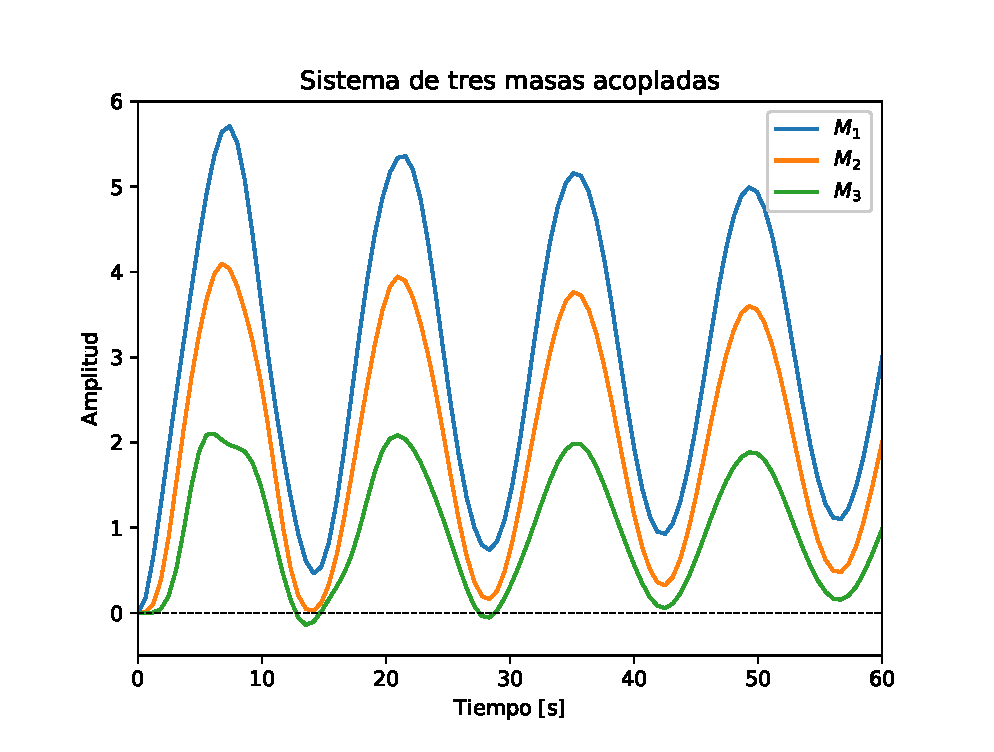
\includegraphics[scale=0.45]{SistemaTresMasasRK4.eps} 
\end{figure}
\end{frame}
\section{Explotando Python para la solución de EDO}
\begin{frame}
\frametitle{Sistema Lotka-Volterra}
Las ecuaciones de Lotka-Volterra, también son conocidas como ecuaciones de depredador-presa, descrito por un sistema de 2 ecuaciones diferenciales no lineales de primer orden, que se utiliza frecuentemente para describir la dinámica de sistemas biológicos donde interaccionan dos especies, un depredador y una de sus presas.
\end{frame}
\begin{frame}
El sistema evoluciona de acuerdo al par de ecuaciones:
\begin{eqnarray*}
\dfrac{du}{dt} &=& au - buv \\
\dfrac{dv}{dt} &=& -cv + dbuv
\end{eqnarray*}
donde:
\fontsize{12}{12}\selectfont
\begin{itemize}
\item $u$ es el número de presas (ej. Conejos)
\item $v$ es el número de depredadores (ej. Zorros)
\item $a$ es la tasa natural de crecimiento de conejos, sin que haya zorros.
\item $b$ es la tasa natural de la muerte de conejos, debido a la depredación.
\item $c$ es la tasa natural de la muerte del zorro, cuando no hay conejos.
\item $d$ es el factor que describe el número de conejos capturados.
\end{itemize}
\end{frame}
\begin{frame}
Vamos a utilizar $X = [u, v]$ para describir el estado de las poblaciones.
\end{frame}
\begin{frame}[fragile]
\frametitle{Definiendo las ecuaciones}
\begin{lstlisting}
from numpy import *
import pylab as p

a = 1.
b = 0.1
c = 1.5
d = 0.75

def dXdt(X, t=0):
    return array([ a*X[0] -   b*X[0]*X[1] ,  -c*X[1] + d*b*X[0]*X[1] ])
\end{lstlisting}
\end{frame}
\begin{frame}[fragile]
\frametitle{Población en equilibrio}
Antes de usar Scipy para integrar el sistema, veremos de cerca la posición de equilibrio. El equilibrio ocurre cuando la tasa de crecimiento es igual a 0, lo que nos da dos puntos fijos:
\begin{lstlisting}
X_f0 = array([     0. ,  0.])
X_f1 = array([ c/(d*b), a/b])
all(dXdt(X_f0) == zeros(2) ) and all(dXdt(X_f1) == zeros(2))
\end{lstlisting}
\end{frame}
\begin{frame}[fragile]
Para usar la función \texttt{odeint}, hay que definir el parámetro de tiempo $t$, así como las condiciones inciales de la población: 10 conejos y 5 zorros.
\begin{lstlisting}
t = linspace(0, 15,  1000)
              
X0 = array([10, 5])         
            
X = integrate.odeint(dXdt, X0, t)
\end{lstlisting}
La función \texttt{odeint} requiere de tres argumentos: la función (o arreglo de funciones), la condición inicial (o arreglo de condiciones iniciales) y el tiempo.
\end{frame}
\begin{frame}[fragile]
Una vez obtenido el código para la solución del problema, ahora nos corresponde graficar el conjunto de datos obtenido, para ello, usamos la siguiente rutina en Python:
\begin{lstlisting}
conejos, zorros = X.T

f1 = p.figure()
p.plot(t, conejos, 'r-', label='Conejos')
p.plot(t, zorros  , 'b-', label='Zorros')
p.grid()
p.legend(loc='best')
p.xlabel('tiempo')
p.ylabel('poblacion')
p.title('Evolucion de la poblacion de conejos y zorros')
p.show()
\end{lstlisting}
\end{frame}
\begin{frame}
\frametitle{Resultado gráfico}
\begin{figure}
	\centering
	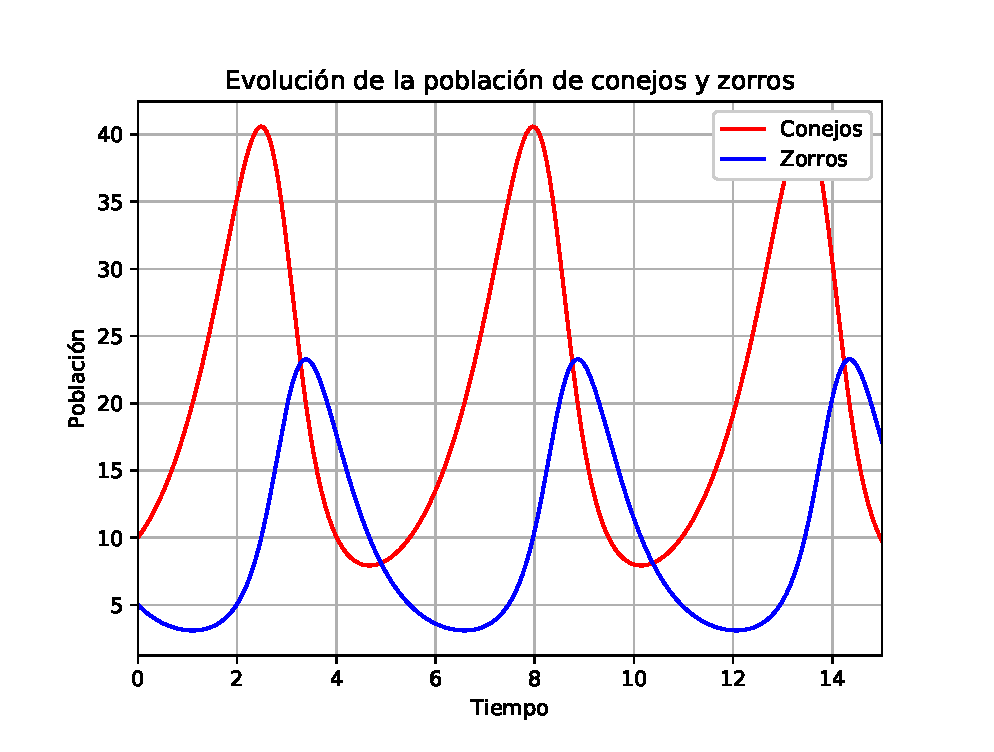
\includegraphics[scale=0.5]{LotkaVolterra_01.eps} 
\end{figure}
\end{frame}
\begin{frame}
La gráfica anterior nos da la información sobre el número tanto de conejos como de zorros durante el intervalo de tiempo estudiado, es decir, tenemos una especie de ''censo''.
\\
\medskip
Para ver la dinámica de las poblaciones propiamente, ahora representamos el espacio fase del sistema, por lo que tenemos que hacer algunos ajustes en el código que usamos anteriormente.
\end{frame}
\begin{frame}[fragile]
Consideremos las condiciones de equilibrio, es decir, donde la tasa de crecimiento es cero:
\begin{lstlisting}
X_f0 = array([     0. ,  0.])
X_f1 = array([ c/(d*b), a/b])
\end{lstlisting}
\end{frame}
\begin{frame}[fragile]
Dibujaremos el espacio fase con algunos elementos visuales con el fin de decoración nada más.
\begin{lstlisting}
values  = linspace(0.3, 0.9, 5)                         

vcolors = p.cm.autumn_r(linspace(0.3, 1., len(values)))  

f2 = p.figure()
\end{lstlisting}
El módulo \texttt{cm} proporciona un gran conjunto de mapas de colores, así como las funciones para crear nuevos mapas de color; existen varios mapas ya definidos: \texttt{autumn, bone, cool, copper, flag, gray, hot, hsv, jet, pink, prism, spring, summer, winter, spectral}.
\end{frame}
\begin{frame}[fragile]
Se van a dibujar ahora las trayectorias para diferentes condiciones iniciales (número de conejos y zorros)
\begin{lstlisting}
for v, col in zip(values, vcolors):
    X0 = v * X_f1
    X = integrate.odeint( dX_dt, X0, t)
    p.plot( X[:,0], X[:,1], lw=3.5*v, color=col, label='X0=(%.f, %.f)' % ( X0[0], X0[1]) )
\end{lstlisting}
La función \texttt{zip} sirve para reorganizar las listas en Python. Como parámetros admite un conjunto de listas. Lo que realmente hace es tomar el elemento i-ésimo elemento de cada lista y los une en una tupla, después une todas las tuplas en una lista.
\\
\medskip
En cada gráfica se modifica el grosor de la línea y el color que se le asocia.
\end{frame}
\begin{frame}[fragile]
Se define una malla y se calcula la dirección
\begin{lstlisting}
ymax = p.ylim(ymin=0)[1]                        
xmax = p.xlim(xmin=0)[1]
nb_points   = 20
 
x = linspace(0, xmax, nb_points)
y = linspace(0, ymax, nb_points)
\end{lstlisting}
\end{frame}
\begin{frame}[fragile]
\begin{lstlisting}
X1 , Y1  = meshgrid(x, y)                       
DX1, DY1 = dX_dt([X1, Y1])                      
M = (hypot(DX1, DY1))                           
M[ M == 0] = 1.                                 
DX1 /= M                                        
DY1 /= M
\end{lstlisting}
Con \texttt{X1} y \texttt{Y1} se crea una malla, con \texttt{DX1} y \texttt{DY1} se calcula el crecimiento de las poblaciones en la malla, \texttt{M} calcula la norma de la tasa de crecimiento, para ello, usa la función\texttt{hypot}, \texttt{M[M==0] =1.} evita que hagamos una división entre cero, \texttt{DX1/M} y \texttt{DY1/M} normaliza cada vector.
\end{frame}
\begin{frame}[fragile]
Se dibujan las direcciones usando \texttt{quiver}
\begin{lstlisting}
p.title('Trayectorias y campo de direccion')
Q = p.quiver(X1, Y1, DX1, DY1, M, pivot='mid', cmap=p.cm.jet)
p.xlabel('Numero de conejos')
p.ylabel('Numero de zorros')
p.legend()
p.grid()
p.xlim(0, xmax)
p.ylim(0, ymax)
p.show()
\end{lstlisting}
La función \texttt{quiver} genera el mapa vectorial, requiere de cinco argumentos: las posiciones X1,Y1 de inicio, el valor de las componentes del vector DX1, DY1 y el color asociado, el argumento \texttt{pivot} indica en qué parte de la malla se va a colocar el vector.
\end{frame}
\begin{frame}
\frametitle{Resultado gráfico}
\begin{figure}
	\centering
	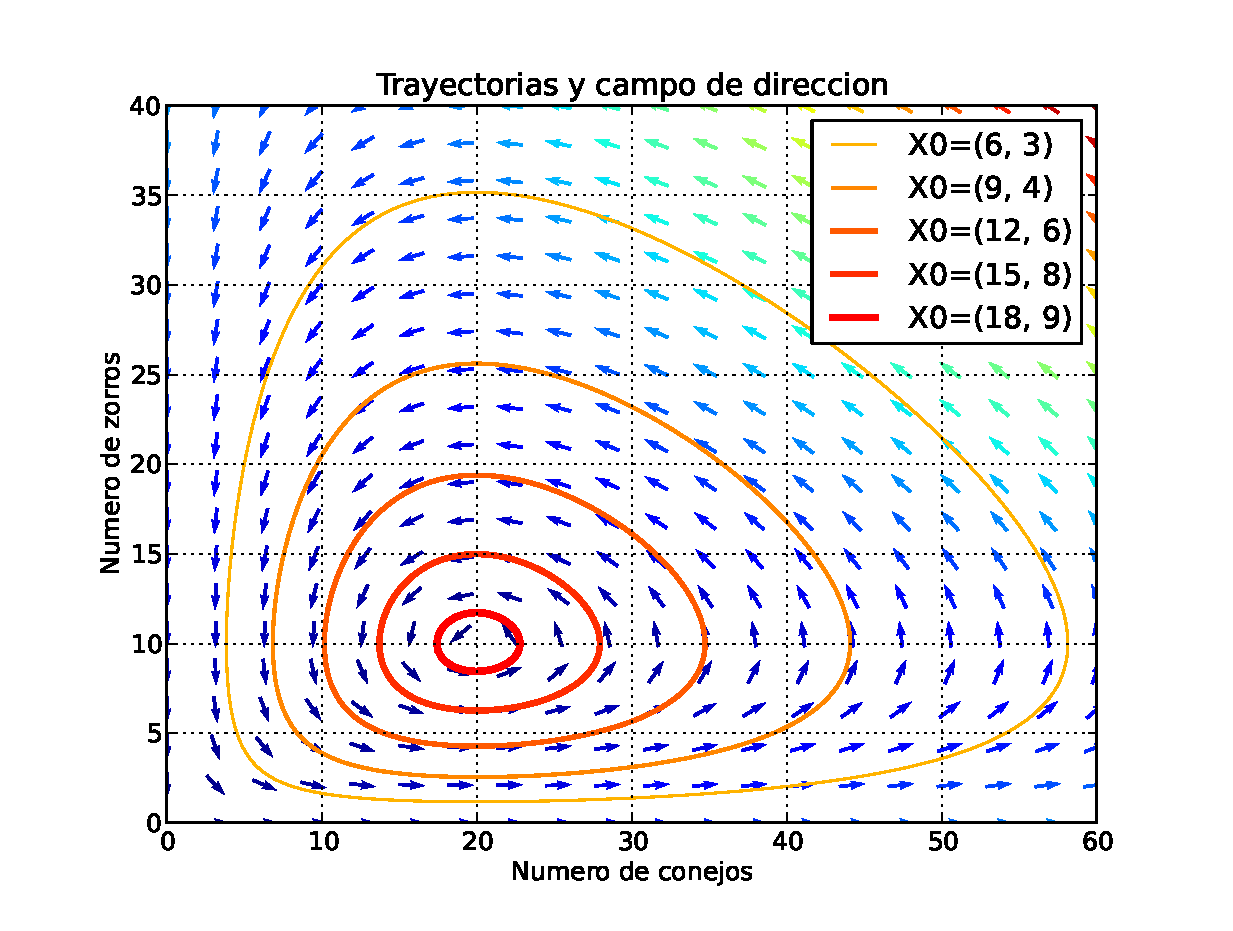
\includegraphics[scale=0.5]{LotkaVolterra_02.eps} 
\end{figure}
\end{frame}
\begin{frame}
\frametitle{Ejercicio para resolver}
El modelo de Lorenz se usa para estudiar la formación de torbellinos en la atmósfera, aunque abordó el problema de manera general, estableció las bases para el estudio de sistemas dinámicos, el conjunto de ecuaciones está dado por
\begin{eqnarray*}
\dfrac{dy_{1}}{dt} &=& a(y_{2}-y_{1}) \\
\dfrac{dy_{2}}{dt} &=& (b - y_{3})y_{1} - y_{2} \\
\dfrac{dy_{3}}{dt} &=& y_{1}y_{2} - cy_{3}
\end{eqnarray*}
en el modelo,$a$, $b$ y $c$ son parámetros positivos. Resuelve este modelo numéricamente, grafica la solución. Utiliza $a = 10$, $b= 28$ y $c=8/3$.
\end{frame}
\begin{frame}
\frametitle{Resultado gráfico}
Usando $a = 10$, $b= 28$ y $c=8/3$
\begin{figure}
	\centering
	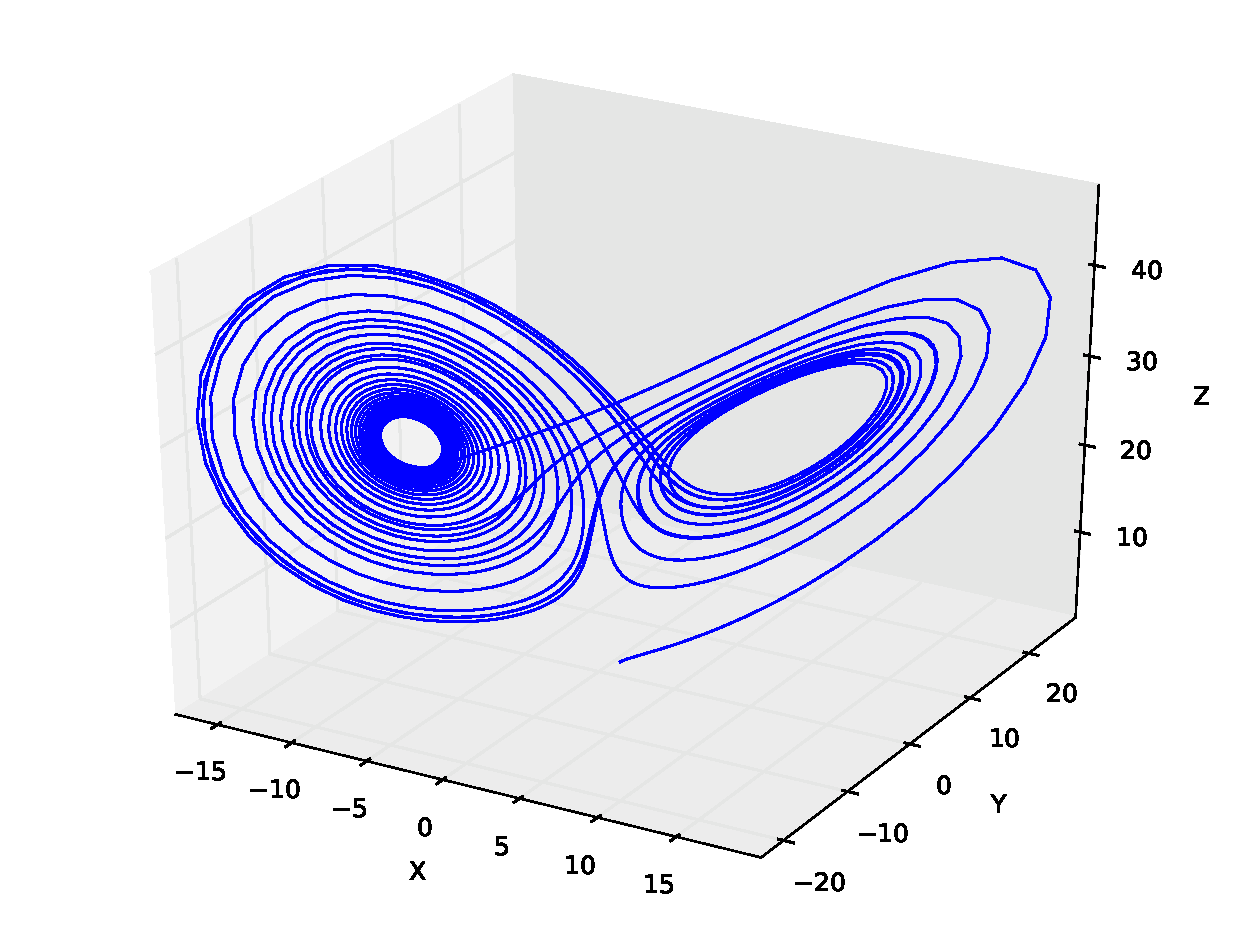
\includegraphics[scale=0.5]{Lorenz_01.eps} 
\end{figure}
\end{frame}
\end{document}